\documentclass[12pt,a4paper]{article}
\usepackage[utf8]{inputenc}
\usepackage[ngerman]{babel}
\usepackage{hyperref}
\usepackage[T1]{fontenc}
\usepackage{amsmath}
\usepackage{amsfonts}
\usepackage{amssymb}
\usepackage{graphicx}
\author{Jonathan Weißenberger}
\title{Projektbeschreibung/Aufgabenbeschreibung}
\begin{document}
\maketitle
\newpage
\tableofcontents
\newpage
\section{Allgemeine Beschreibung}
Das Team, bestehend aus Alexander Hebel, Dennis Seilnacht und Jonathan Weißenberger beschäftigen sich im vierten Semester mit der Portierung der Umgebung OpenPEARL für Microcontroller. Das Target in der Portierung ist das Entwicklungsboard STM32F746-DISCO. Zusätzlich zur Portierung erfolgt eine Demoapplikation. Hierbei ist die bereits existierende Kugelsortierungsanlage der Hochschule Furtwangen mit dem Microcontrollerboard zu steuern.
\begin{figure}[h]
\begin{center}
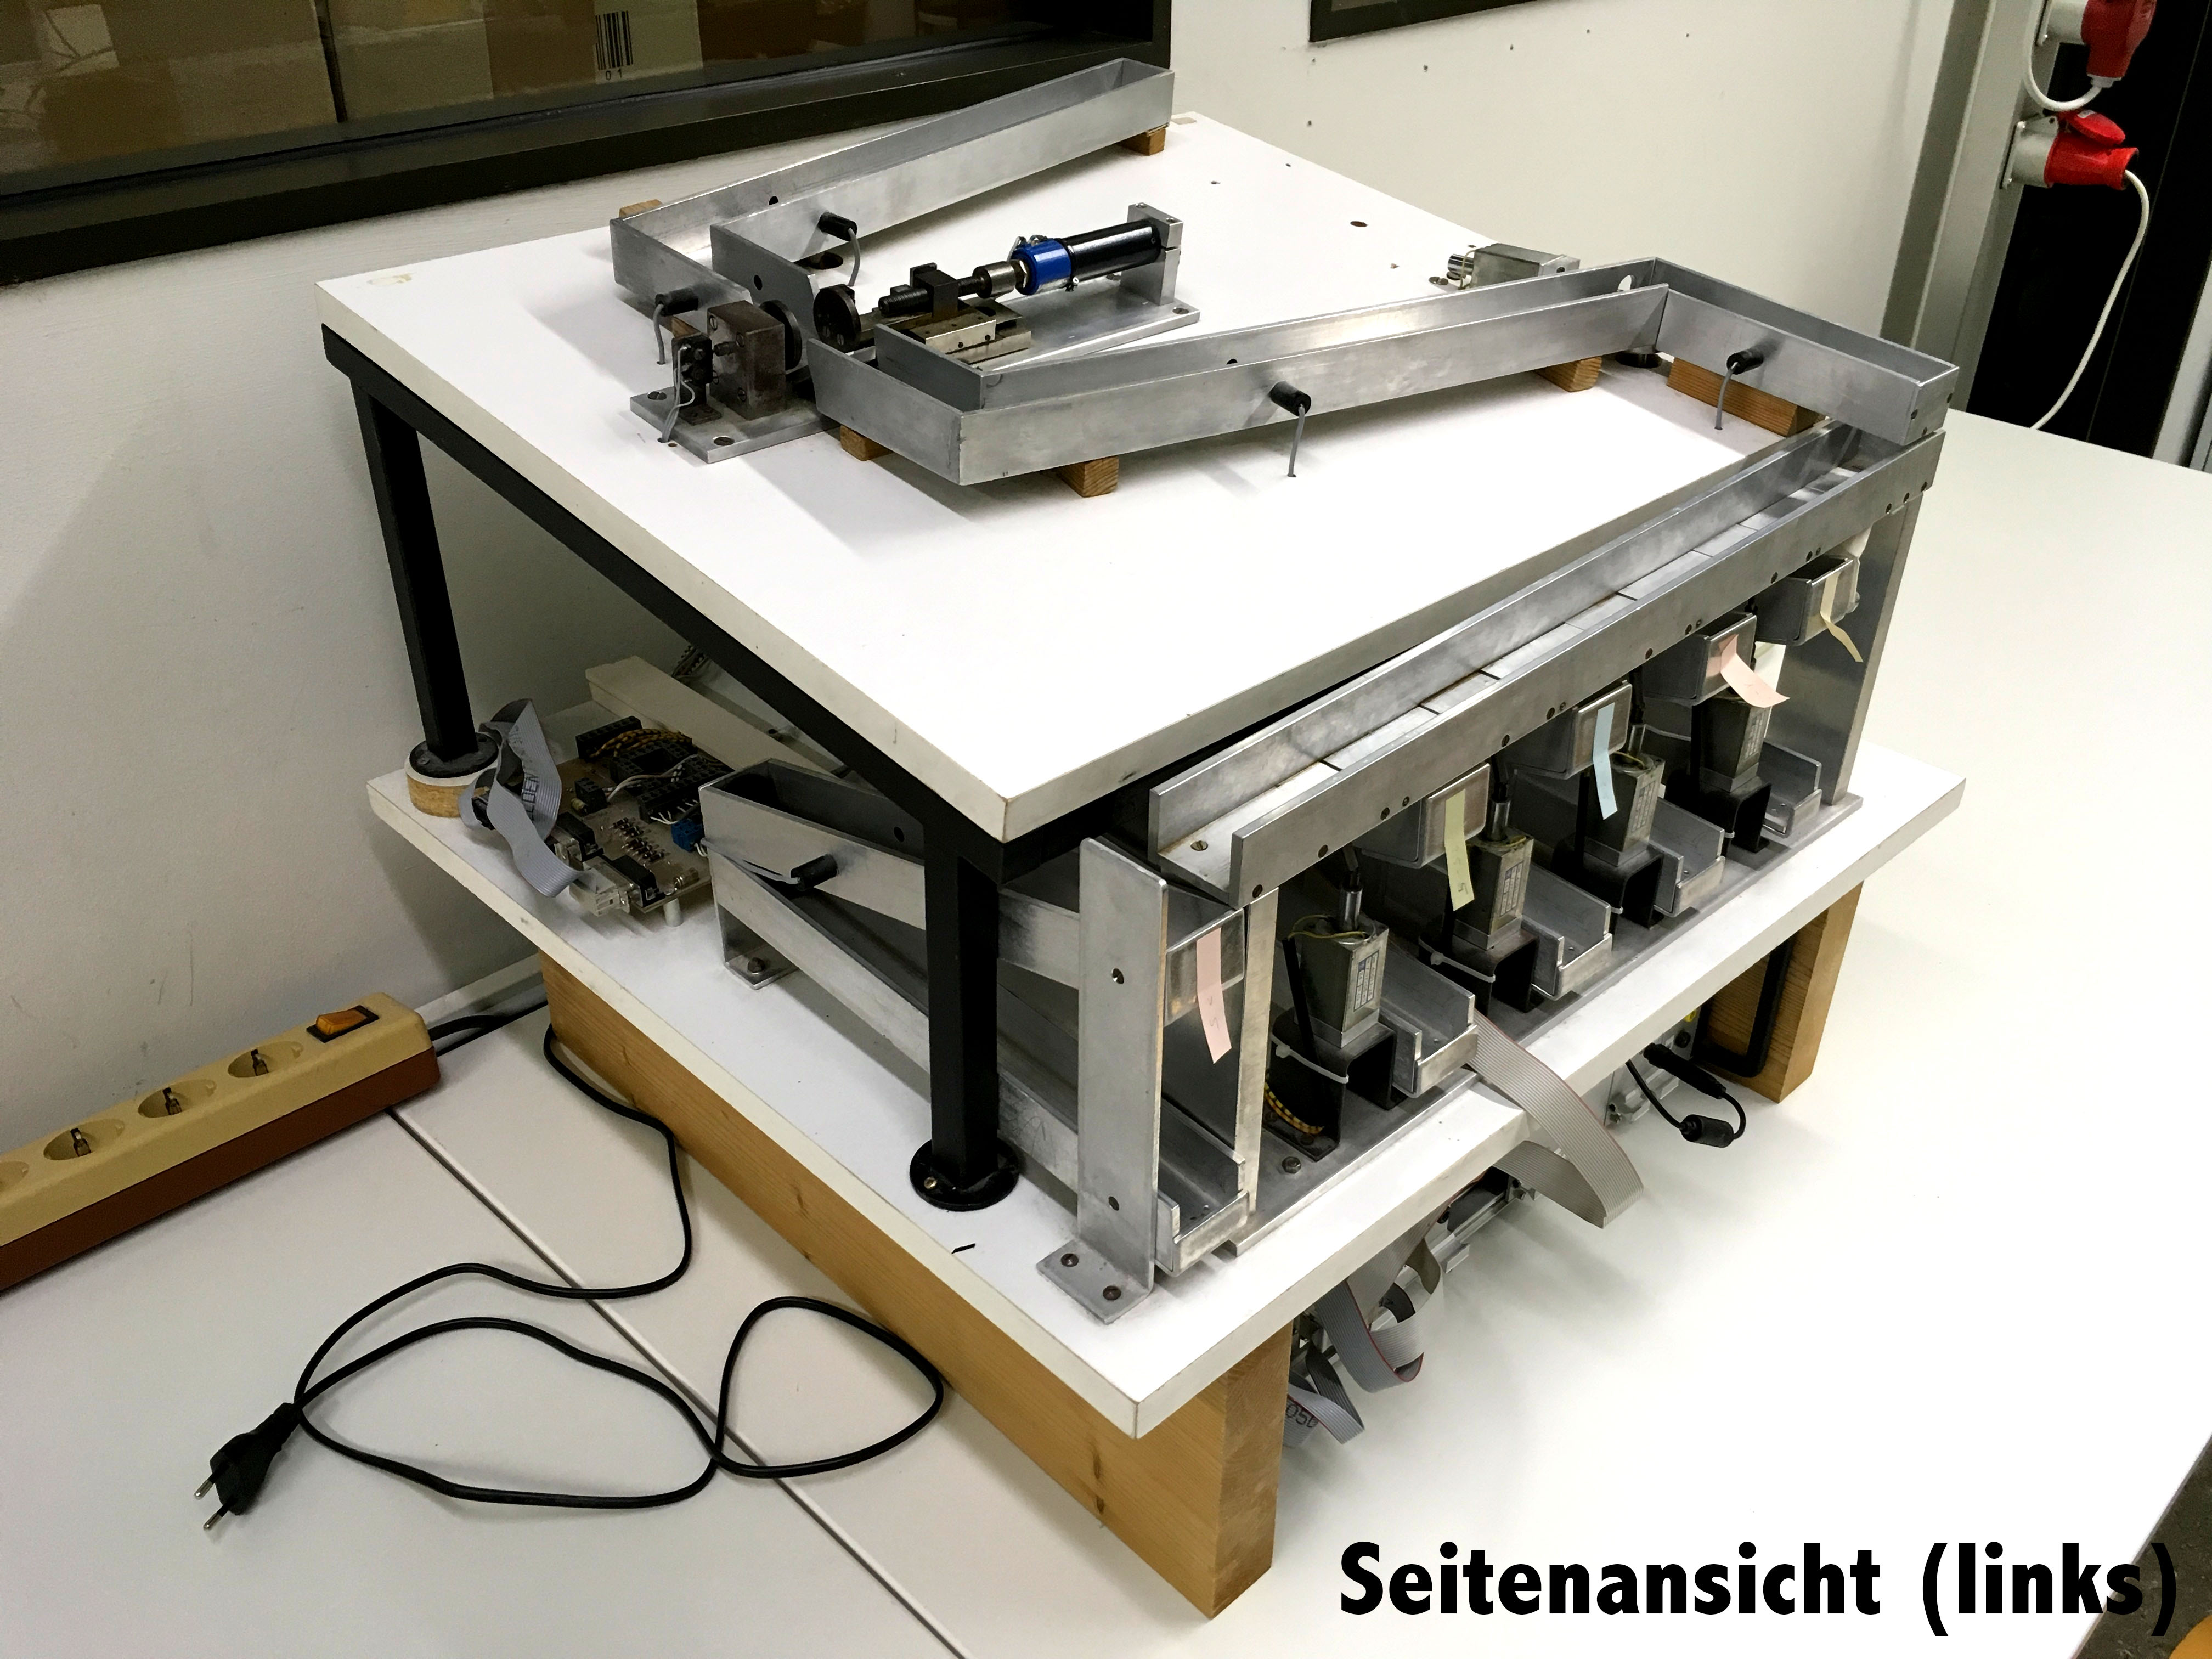
\includegraphics[width=10cm]{grafiken/Seitenansicht.jpg}
\label{bild_kugelsortiermaschine}
\caption{Kugelsortiermaschine}
\end{center}
\end{figure}
Das primäre Ziel der Arbeit ist die Lauffähigkeit von OpenPEARL auf der Zielplattform. Im Konkreten bedeutet das, dass Software in der Sprache OpenPEARL übersetzt werden kann und dann nach der Übertragung auf dem Zielsystem läuft. Das Kompilat soll nachvollziehbare Ergebnisse liefern, die wir zuvor definieren. Im Fall der Sortierungsanlage sollen die Kugeln ihrer jeweiligen Dichte entsprechend in die einzelnen Fächer eingeordnet werden. Die Dichte errechnet sich dann aus dem Durchmesser der Kugel und dem Gewicht ($Dichte=Masse/Volumen$). Zu den Funktionalitäten, die mit OpenPEARL genutzt werden sollen gehört das $I^2C$-Bussystem. Durch das Bussystem wird die Kugelsortierungsmaschine angesteuert und Informationen abgerufen. Außerdem soll eine Kommunikationsverbindung mit dem Target mittels UART-Schnittstelle von einem Host-Computer aus möglich sein. Durch die Schnittstelle soll es möglich sein, Befehle an den Microcontroller zu senden und Informationen abzurufen. 
\begin{figure}[h]
\begin{center}
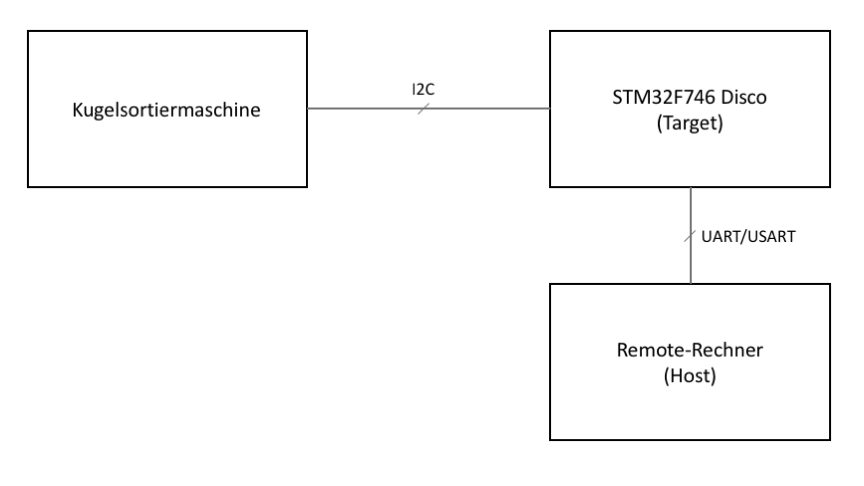
\includegraphics[width=10cm]{grafiken/Schematik.png}
\caption{Schematik des Projektaufbaus}
\label{schematik_projektaufbau}
\end{center}
\end{figure}
Sofern die Grundfunktionalitäten in angemessener Zeit umgesetzt werden können, wird zusätzlich die Verwendbarkeit des Displays angestrebt. Das Display soll zusätzlich Statusberichte liefern über den Zustand der Sortierungsanlage. 
\subsection{Beschreibung der Kugelsortiermaschine}
Die Sortiermaschine wird von der Hochschule Furtwangen bereitgestellt. In diesem Abschnitt wird im Wesentlichen die Funktionalität und die Bestandteile der Sortiermaschine geklärt.
Der Einwurf der Kugeln erfolgt von Hand. In der Draufsicht (siehe Abbildung), ist die Laufbahn, die Ballführung zu erkennen. Dadurch, dass die Führung leicht abschüssig ist, rollen die Kugeln. Auf dem Weg nach unten, passieren die Kugeln mehrere Lichtschranken. Durch diese Lichtschranken ist es möglich, die Schienen in Abschnitte einzuteilen und mehrere Kugeln gleichzeitig erfassen zu können. Wenn beispielsweise eine Kugel Lichtschranke 3 passiert, kann im Balleinwurf schon eine neue Kugel eingegeben werden. Die Durchmesserbestimmung ist im wesentlichen ein Motor, der eine Gewindestange in Richtung Rollbahn bewegt. Nachdem eine Kugel eingeworfen wurde, rollt diese als erstes in Richtung dieser Messeinheit. Durch eine Klappe von unten wird die Kugel an der Messstation gestoppt. Wie bereits beschrieben, wird die Gewindestange dann in Richtung Rollfeld gedreht, bis ein Taster ausgelöst wird. Anschließend daran, wird der Potentiometerwert ausgelesen. Bei dem Potentiometer handelt es sich um einen Drehpotentiometer, dessen Widerstandswert sich mit dem Drehen der Gewindestange verändert. Anhand dieses Wertes kann der Durchmesser der Kugel bestimmt werden. Ist der Wert gelesen, wird die Gewindestange zurückgefahren und die Bodenklappe lässt den Ball weiterrollen. Die nächste Station, die von der Kugel passiert wird ist die Waageeinheit. Sie ermittelt das Gewicht der Kugel. Durch eine Kule auf der Waagefläche bleibt die Kugel auf der Waage liegen. Sobald der Wert gelesen ist, wird die Kugel durch einen Bolzen herausgeschossen. Anhand der ermittelten Dichte wird dann bestimmt, welche Klappe sich öffnet. Die jeweilige Klappe bestimmt darüber, in welchem Fach die Kugel landet.
\begin{figure}[h]
\begin{center}
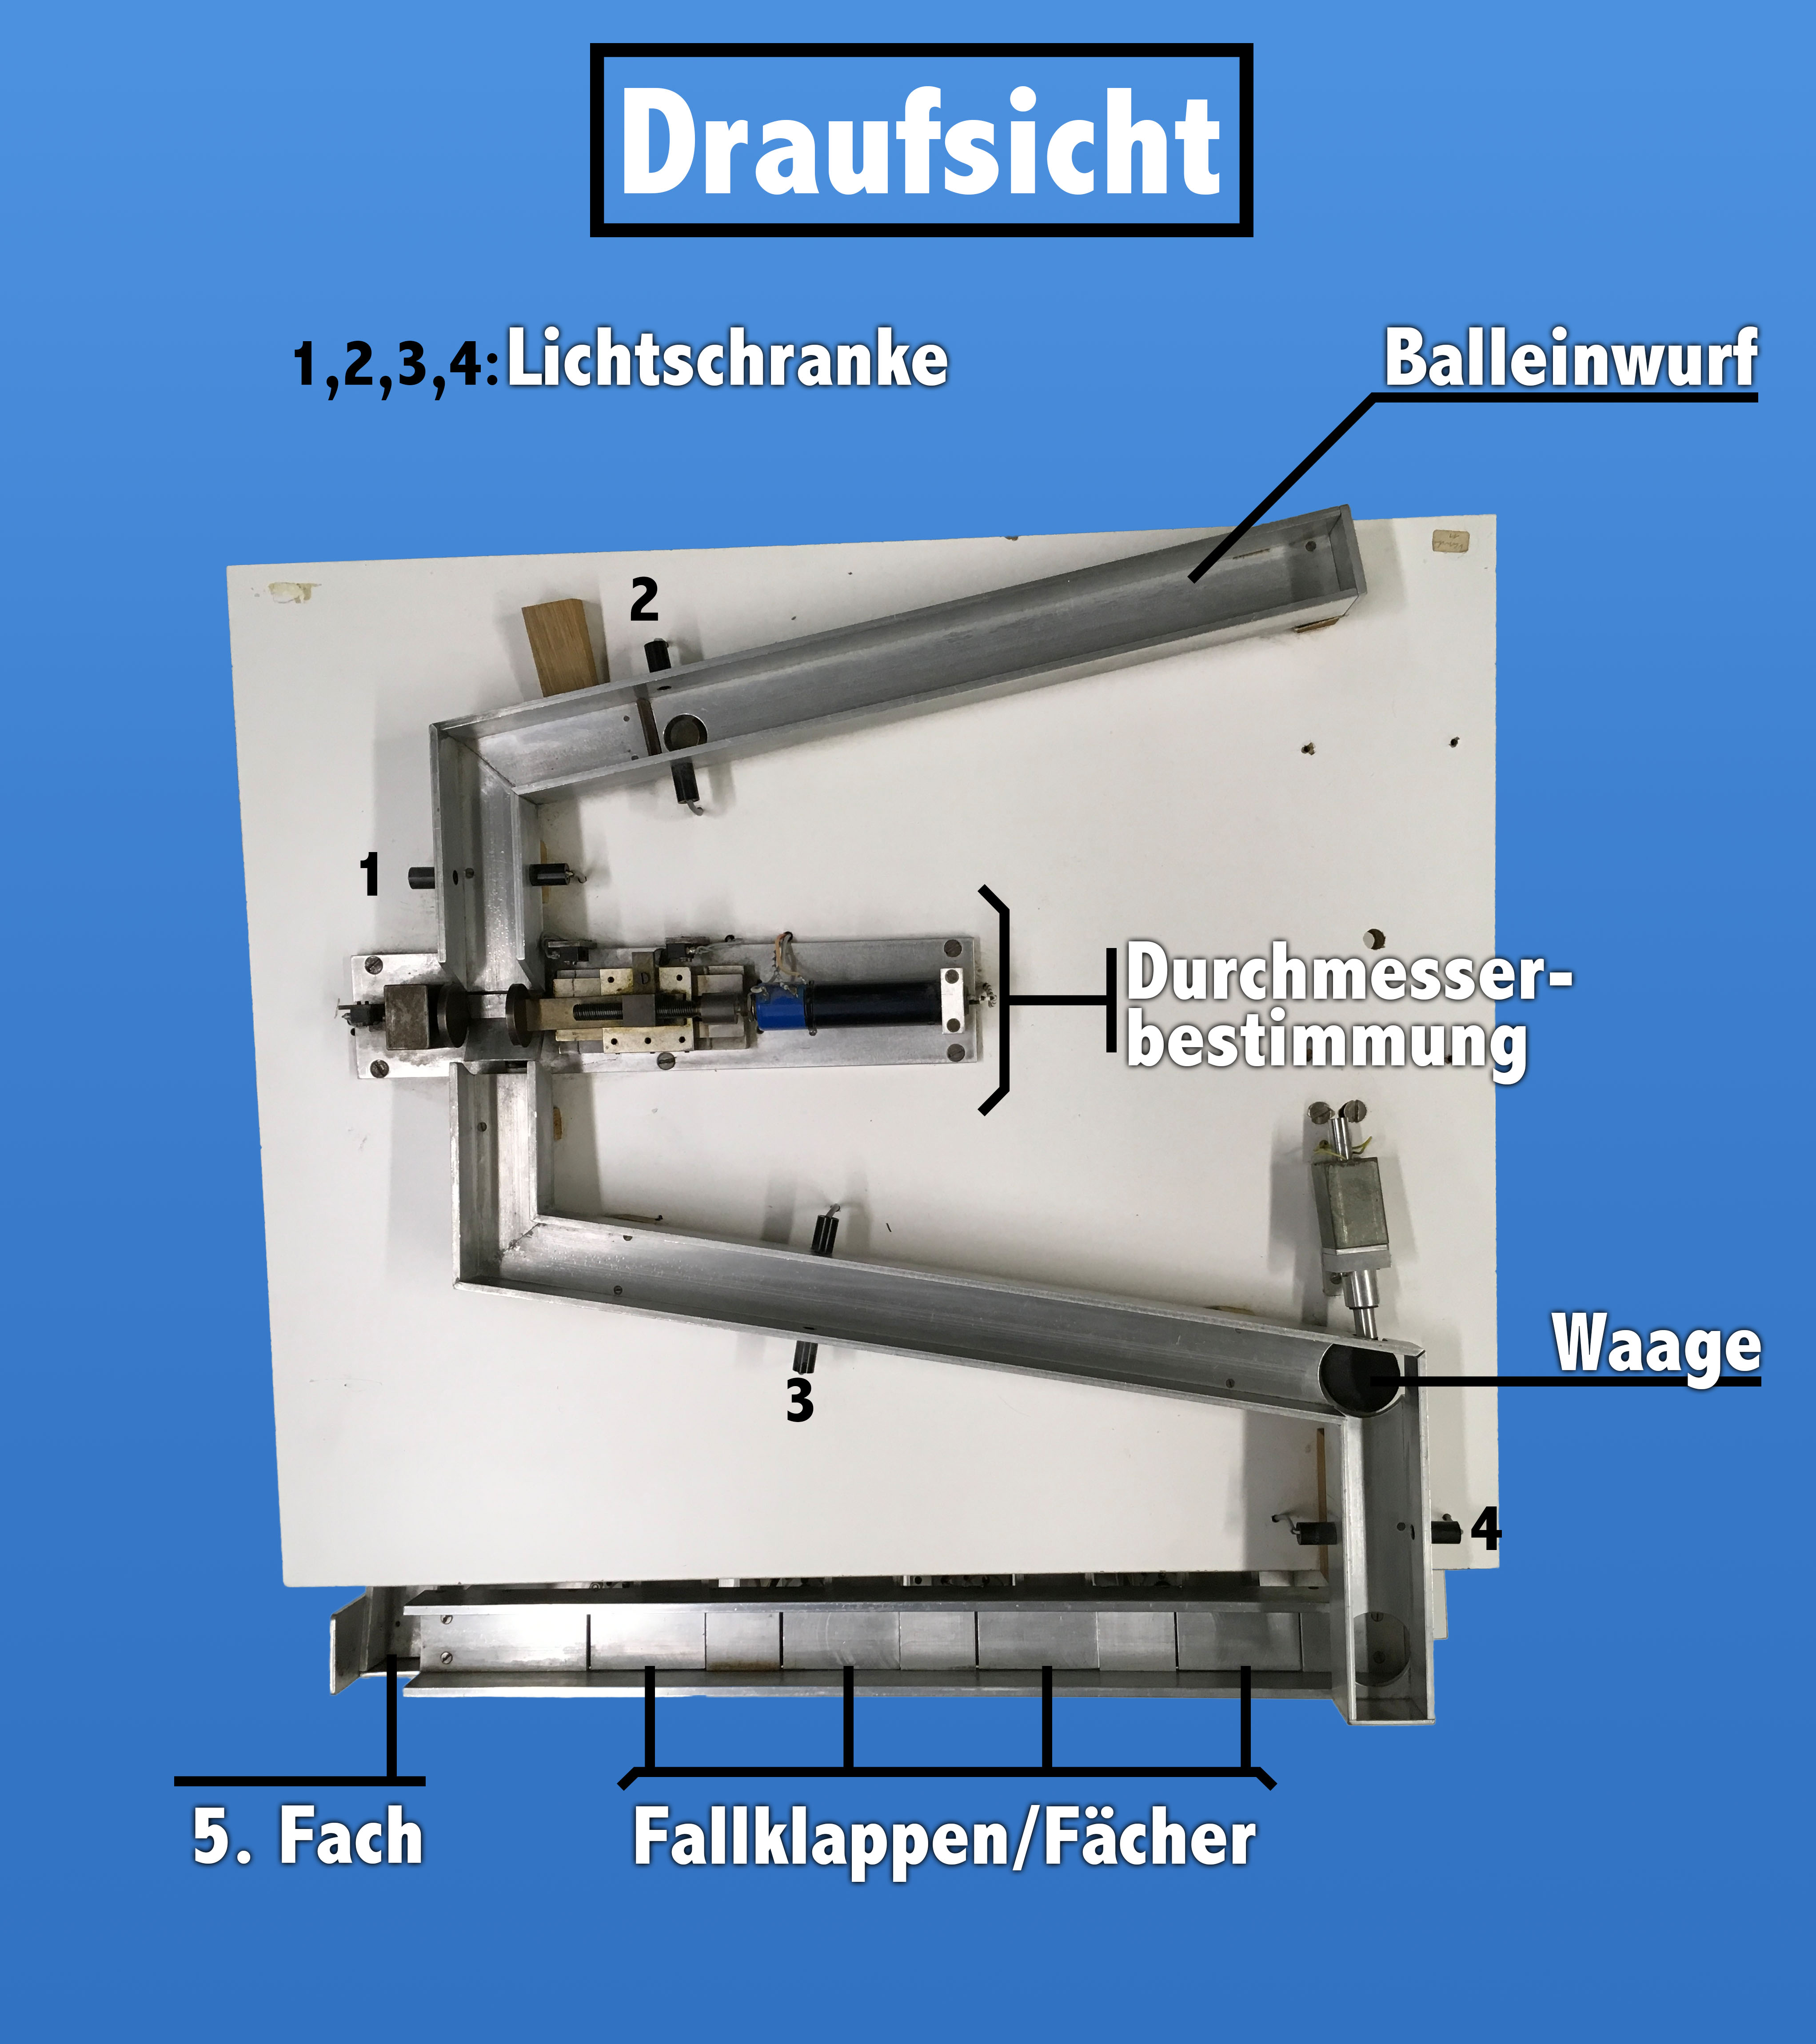
\includegraphics[width=12cm]{grafiken/Draufsicht.jpg}
\caption{Die Draufsicht auf die Demoapparatur}
\label{draufsicht_sortiermaschine}
\end{center}
\end{figure}

\subsection{Beschreibung des Zeitplans}
Der ausgearbeitete Zeitplan war erst erstellbar nach den ersten Wochen. Nach dieser Zeit war schon Toolchain, Debuggerinstallation, Testprogrammausführung vollendet. 
\begin{figure}[h]
\begin{center}
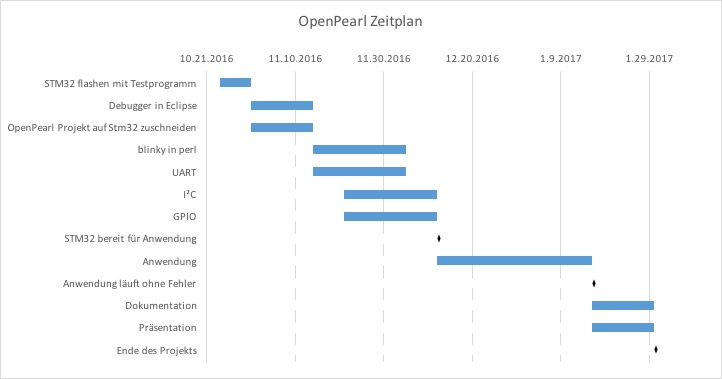
\includegraphics[width=13.5cm]{grafiken/zeitplan.jpg}
\caption{Zeitplan als Ergebnis des Meetings am 09.11.2016}
\label{zeitplan}
\end{center}
\end{figure}

\end{document}